\documentclass{beamer}

\usepackage{helvet}
\usepackage{hyperref, graphicx}
\usepackage{amsthm}
\usepackage{etoolbox}
%\usepackage{multicol}
\usepackage{tikz}
\usepackage{ulem}

\usetheme{default}
\setbeamertemplate{navigation symbols}{}
\AtBeginSection[ ]
{
\begin{frame}{Outline}
    \tableofcontents[currentsection]
\end{frame}
}

% Default fixed font does not support bold face
\DeclareFixedFont{\ttb}{T1}{txtt}{bx}{n}{11} % for bold
\DeclareFixedFont{\ttm}{T1}{txtt}{m}{n}{12}  % for normal - use in headings

% Custom colors
\usepackage{color}
\definecolor{TUGray}{RGB}{101,101,137}
\definecolor{TUBlack}{RGB}{30,0,0}
\definecolor{mygreen}{RGB}{45,111,63}
\definecolor{keywords}{RGB}{205,114,0}
\definecolor{comments}{RGB}{181,51,139}
\definecolor{strings}{RGB}{58,144,81}
\definecolor{numeric}{RGB}{66,110,176}
\definecolor{linos}{rgb}{0.4,0.4,0.4}
\definecolor{links}{rgb}{0,0.4,0.75}

\definecolor{bggray}{RGB}{232, 233, 235}

\usecolortheme[named=mygreen]{structure}
\setbeamercolor{normal text}{fg=TUBlack}\usebeamercolor*{normal text}

\setbeamercolor{codecol}{fg=TUGray!25!black,bg=bggray}

\hypersetup{colorlinks, linkcolor=links, urlcolor=links}

\usepackage[T1]{fontenc}
\usepackage[sfdefault,scaled=.85]{FiraSans}
\usepackage{mathpazo}

\usepackage{listings}

\newtoggle{InString}{}% Keep track of if we are within a string
\togglefalse{InString}% Assume not initally in string

\newcommand\digitstyle{\color{numeric}}
\makeatletter
\newcommand{\ProcessDigit}[1]
{%
  \ifnum\lst@mode=\lst@Pmode\relax%
   {\digitstyle #1}%
  \else
    #1%
  \fi
}
\makeatother

\lstset{literate=%
    {0}{{{\ProcessDigit{0}}}}1
    {1}{{{\ProcessDigit{1}}}}1
    {2}{{{\ProcessDigit{2}}}}1
    {3}{{{\ProcessDigit{3}}}}1
    {4}{{{\ProcessDigit{4}}}}1
    {5}{{{\ProcessDigit{5}}}}1
    {6}{{{\ProcessDigit{6}}}}1
    {7}{{{\ProcessDigit{7}}}}1
    {8}{{{\ProcessDigit{8}}}}1
    {9}{{{\ProcessDigit{9}}}}1
	{<=}{{\(\leq\)}}1
	{>=}{{\(\geq\)}}1,
	% morestring=[b]",
    % morestring=[b]',
    % morecomment=[l]{//},
}

\lstdefinelanguage{Pseudo}{
    morekeywords={return, while, if, for, input},
    morecomment=[l]{\#},
}

% Pseudocode style
\newcommand\pseudostyle{\lstset{
language=Pseudo,
basicstyle=\fontfamily{ccr}\scriptsize,
commentstyle=\it\scriptsize\color{linos},
keywordstyle=\it\bfseries\scriptsize,
mathescape=true,
literate=
    {=}{$\leftarrow{}$}{1}
    {==}{$={}$}{1}
    {<=}{{\(\leq\)}}1
	{>=}{{\(\geq\)}}1,
xleftmargin=18pt,
xrightmargin=4pt,
aboveskip=12pt,
belowskip=0pt,
frame=tB,
keepspaces=true
}}

% Python style for highlighting
\newcommand\pythonstyle{\lstset{
language=Python,
basicstyle=\ttfamily\tiny,
numbers=left,
numberstyle=\tiny\color{linos},
morekeywords={self, np},              % Add keywords here
keywordstyle=\tiny\color{keywords},
commentstyle=\it\tiny\color{comments},    % Custom highlighting style
stringstyle=\tiny\color{strings},
xleftmargin=18pt,
xrightmargin=4pt,
aboveskip=0pt,
belowskip=0pt,
escapeinside={(*@}{@*)},
frame=l,                         % Any extra options here
showstringspaces=false,
keepspaces=true
}}

% Pseudocode environment
\lstnewenvironment{pseudo}[1][]
{
    \pseudostyle
    \lstset{
        #1
    }
}
{}

% Python environment 
\lstnewenvironment{python}[1][]
{
	\pythonstyle
	\lstset{
	#1
	}
}
{}

% wrap the Python environment
\newenvironment{codeblock}
    {\hfill\begin{beamerboxesrounded}[lower=codecol, width=0.8\textwidth]
    \medskip

    }
    { 
    \end{beamerboxesrounded}\hfill
    }

\theoremstyle{example}
\newtheorem{question}{Question}

\newcommand{\ct}[1]{\lstinline[language=Python,basicstyle=\ttfamily\footnotesize,stringstyle=\small\color{strings}]!#1!}
\newcommand{\ttt}[1]{{\small\texttt{#1}}}
\newcommand{\lsitem}[2]{\ttt{{#1}[}\ct{#2}\ttt{]}}

\author{Chris Cornwell}
\date{October 21, 2025}
\title{Classification tasks, the Perceptron model}

\begin{document}

\begin{frame}
\titlepage
\end{frame}

\begin{frame}
\frametitle{Outline}
\tableofcontents
\end{frame}

\section{Classification tasks}

%%%%
\begin{frame}
\frametitle{Example of Classification}
Use some model to determine a digit that was (hand)written in an image
\begin{center}

\includegraphics[height=0.25\textheight]{../../Images/50.png}
\end{center}\vspace*{-8pt}

$\leadsto$ \hspace*{0.6in} \ct{0, 1, 2, 3, 4, 5, 6, 7, 8,} or \ct{9}.

\pause
\begin{itemize}
    \item Convert image to a vector (\textit{in some way}) $\to\ {\bf x}$.
    \item Your model's output: the (predicted) digit. 
\end{itemize}

\pause
In data provided, $\{({\bf x}_i, y_i)\}$, observed (``correct'') label is $y_i\in\{0,1,\ldots,9\}$.

\pause 
Value of $y$ is on number line; but, consider it a \emph{label} (or, one of a few separate ``buckets'') used to organize different points ${\bf x}$. (When $y_i=5$, predicting $4$ is not any better than $0$.)

\end{frame}

%%%%
\begin{frame}
\frametitle{Close only counts in \sout{horseshoes} \ldots Regression}
In linear regression, on indpt.\ variables $x_1,x_2,\ldots,x_{N}$, had (affine) linear function $y \approx b + w_1x_1+w_2x_{2}+\ldots+w_{N}x_{N}$; \newline 
values of function $\leftrightarrow$ prediction $\hat{y}$; error term $\varepsilon = y - \hat{y}$.

\pause
In regression, the \textbf{linear model} ${\bf x} \mapsto \hat{y}$ approximates the relationship ${\bf x} \mapsto y$.\footnote{Should consider the output $y$ here to be a random variable, with distribution that depends on ${\bf x}$.} We expect that $|y - \hat{y}|$ is \emph{almost never} exactly 0; a good model: one where $|y - \hat{y}|$ is small on average (but, still positive).

\pause 
``Classification'' tasks: the value $y$ is a label, might not even be a number. The prediction $\hat{y}$ is either wrong, or not wrong; close doesn't count. Good model: when
$\hat{y} = y$ as often as possible.
\end{frame}

\section{Perceptron model}

%%%%
\begin{frame}
\frametitle{A linear model for classification}
    \textbf{Binary classification:} Data from $\mathbb R^N$ for some $N>0$ and only two labels, $\{1, -1\}$. %(e.g., this is Spam (\texttt{S}) or it is Not spam (\texttt{N})). 
    \pause

    A \emph{hyperplane} in $\mathbb R^N$ is an (affine) linear subspace that separates $\mathbb R^N$ in two. %Perhaps we get lucky and can find a hyperplane $H$ so that data points with label \texttt{S} are on one side of $H$ and data with label \texttt{N} are on the other side.
        Given numbers $w_1,w_2,\ldots,w_d$, and $b$, it can be thought of as the set of points ${\bf x}\in\mathbb R^N$ where the linear function $y=b+w_1x_1+\ldots + w_Nx_N$ has value zero\footnote{Notation here is that $x_1,\ldots,x_N$ are the coordinates of the vector ${\bf x}$.}: 
            \[\{(x_1,\ldots,x_N)\ :\ w_1x_1 + w_2x_2\ldots + w_dx_d + b = 0\}.\]

    \pause
    \begin{figure}[h!]
        \centering
        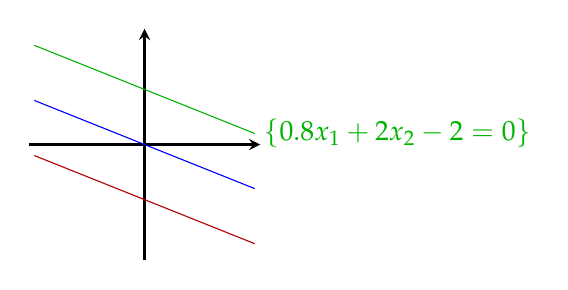
\begin{tikzpicture}[>=stealth, scale=0.7]
            %\fill[blue!35!white, opacity = 0.2] (-4, 3) -- (5, 3) -- (5, -3) -- (2, -3)-- cycle;
            %\fill[red!35!white, opacity = 0.2] (-4, 3) -- (-5, 3) -- (-5, -3) -- (2, -3)-- cycle;
            \draw[thick, ->] (-2.1, 0)-- (2.1, 0); 
            \draw[thick, ->] (0, -2.1) -- (0, 2.1); 
            %\draw[very thick] (-4, 3) -- (2, -3); % node[above right]{\small $H = \{x + y + 1 = 0\}$}; 
            \draw[blue] (-2,0.8) -- (2,-0.8);
            \draw[green!70!black] (-2,1.8) --node[at end, right]{$\{0.8x_1+2x_2-2=0\}$} (2,0.2);
            \draw[red!70!black] (-2,-0.2) -- (2,-1.8);
        \end{tikzpicture}
        \caption{A few hyperplanes in $\mathbb R^2$.}
        \label{figure:hyperplanes}
    \end{figure}

\end{frame}

%%%%
\begin{frame}
    \frametitle{A linear model for classification}
    \textbf{Binary classification:} Data is from $\mathbb R^N$ for some $N>0$ and we only have two labels, $\{1, -1\}$. %(e.g., this is Spam (\texttt{S}) or it is Not spam (\texttt{N})). 
        
        A \emph{hyperplane} in $\mathbb R^N$ is an (affine) linear subspace that separates $\mathbb R^N$ in two. %Perhaps we get lucky and can find a hyperplane $H$ so that data points with label \texttt{S} are on one side of $H$ and data with label \texttt{N} are on the other side.
        Given numbers $w_1,w_2,\ldots,w_d$, and $b$, it can be thought of as the set of points ${\bf x}\in\mathbb R^N$ where the linear function $y=b+w_1x_1+\ldots + w_Nx_N$ has value zero\footnote{Notation here is that $x_1,\ldots,x_N$ are the coordinates of the vector ${\bf x}$.}: 
            \[\{(x_1,\ldots,x_N)\ :\ w_1x_1 + w_2x_2\ldots + w_dx_d + b = 0\}.\]

    \begin{itemize}
        \item Calling the hyperplane $H$ and rewriting this in vector form: if ${\bf w}=(w_1,w_2,\ldots,w_N)$ and $\tilde{\bf w} = (b,w_1,\ldots,w_N)$, then $H$ is the set of ${\bf x}$ so that $\tilde{\bf x}^\top\tilde{\bf w} = {\bf w}\cdot{\bf x} + b = 0$.
        \pause
        \item $H$ separates $\mathbb R^N$ into two parts: those ${\bf x}$ where ${\bf w}\cdot{\bf x} + b$ is positive and those where ${\bf w}\cdot{\bf x} + b$ is negative.
        \pause
        \item ${\bf w}$ is a vector that is orthogonal to $H$ (which is $(N-1)$-dimensional); $|b|$ and $\lVert{\bf w}\rVert$ relate to how far $H$ is translated away from the origin.
    \end{itemize}
    \vfill

\end{frame}

%%%%
\begin{frame}
\frametitle{Half-space model}
    Using the notation from last slide:  a \emph{half-space model} in $\mathbb R^N$ is determined by $\tilde{\bf w} = (b,w_1,w_2,\ldots,w_N)$, with a corresponding hyperplane $H$.
    
    \pause
    Given ${\bf x}\in \mathbb R^N$, the half-space model can be though of as a function: $h:\mathbb R^d\setminus H \to \{1,-1\}$, with 
    \pause
    \begin{itemize}
        \item (Positive side) set $h({\bf x}) = 1$ if ${\bf w}\cdot{\bf x}+b > 0$.
        \item (Negative side) set $h({\bf x}) = -1$ if ${\bf w}\cdot{\bf x}+b < 0$. 
    \end{itemize}

    \pause
    Given data with labels $y_i = \{\pm1\}$, if there exists a hyperplane $H$ so that, for all $i$, ${\bf x}_i$ has label $1$ if and only if it is on the positive side of $H$, these data are called \textbf{linearly separable}. 

\end{frame}

%%%%
\begin{frame}
    \frametitle{Linearly separable}
    \begin{figure}[h!]
        \centering
        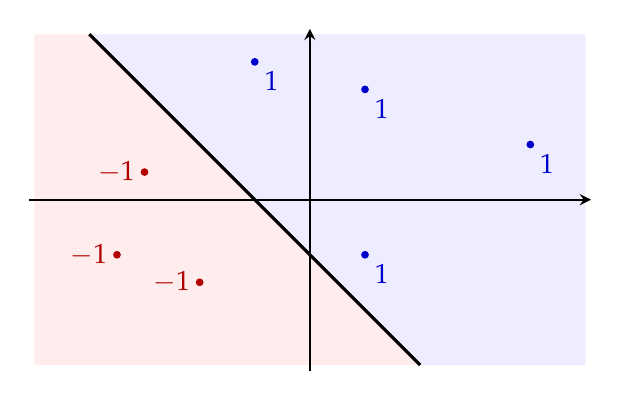
\begin{tikzpicture}[>=stealth, scale=0.7]
            \fill[blue!35!white, opacity = 0.2] (-4, 3) -- (5, 3) -- (5, -3) -- (2, -3)-- cycle;
            \fill[red!35!white, opacity = 0.2] (-4, 3) -- (-5, 3) -- (-5, -3) -- (2, -3)-- cycle;
            \draw[thick, ->] (-5.1, 0)-- (5.1, 0); 
            \draw[thick, ->] (0, -3.1) -- (0, 3.1); 
            \draw[very thick] (-4, 3) -- (2, -3); % node[above right]{\small $H = \{x + y + 1 = 0\}$}; 
            \fill[blue!80!black] (1, 2)node[below right]{$1$} circle (2pt); 
            \fill[blue!80!black] (-1, 2.5)node[below right]{$1$} circle (2pt); 
            \fill[blue!80!black] (1, -1)node[below right]{$1$} circle (2pt); 
            \fill[blue!80!black] (4, 1)node[below right]{$1$} circle (2pt); 
            \fill[red!70!black] (-3, 0.5)node[left]{$-1$} circle (2pt); 
            \fill[red!70!black] (-3.5, -1)node[left]{$-1$} circle (2pt); 
            \fill[red!70!black] (-2, -1.5)node[left]{$-1$} circle (2pt); 
        \end{tikzpicture}
        \caption{The hyperplane $H = \{(x_1,x_2)\in \mathbb R^2: x_1+ x_2+ 1 = 0\}$, corresponding positive and negative regions, ${\bf w} = (1, 1)$, $b = 1$}
        \label{figure:R2HyperplaneLabeled}
    \end{figure}
\end{frame}

%%%%
\begin{frame}
    \frametitle{Not linearly separable}
    \begin{figure}[h!]
        \centering
        \begin{tikzpicture}[>=stealth, scale=0.7]
            %\fill[blue!35!white, opacity = 0.2] (-4, 3) -- (5, 3) -- (5, -3) -- (2, -3)-- cycle;
            %\fill[red!35!white, opacity = 0.2] (-4, 3) -- (-5, 3) -- (-5, -3) -- (2, -3)-- cycle;
            \draw[thick, ->] (-5.1, 0)-- (5.1, 0); 
            \draw[thick, ->] (0, -3.1) -- (0, 3.1); 
            %\draw[very thick] (-4, 3) -- (2, -3); % node[above right]{\small $H = \{x + y + 1 = 0\}$}; 
            \fill[blue!80!black] (1, 2)node[below right]{$1$} circle (2pt); 
            \fill[red!70!black] (1, -1)node[below right]{$-1$} circle (2pt); 
            \fill[red!70!black] (-3, 0.5)node[left]{$-1$} circle (2pt); 
            \fill[blue!80!black] (-2, -1.5)node[left]{$1$} circle (2pt); 
        \end{tikzpicture}
        \caption{A data set in $\mathbb R^2$ that is not linearly separable.}
        \label{figure:notseparable}
    \end{figure}
    \pause
    \begin{itemize}
        \item A criterion (checkable, in theory) that is equivalent to ``not linearly separable''?
    \end{itemize}
\end{frame}

\section{Perceptron algorithm}

%%%%
\begin{frame}
    \frametitle{Setup for Perceptron algorithm}
    Labeled data: $({\bf x}_1, y_1), \ldots, ({\bf x}_P, y_P)$, with ${\bf x}_i\in\mathbb R^N$ and $y_i\in\{\pm1\}$ for all $i$.

    Assuming labeled data is linearly separable, the Perceptron algorithm is a procedure that is guaranteed to find a hyperplane that separates the data.\footnote{Introduced in \textit{The perceptron: A probabilistic model for information storage and organization in the brain}, F.~Rosenblatt, Psychological Review \textbf{65} (1958), 386{--}407.}
    
    \pause
    To describe it: for each ${\bf x}_i$, use the notation $\tilde{\bf w}$ and $\tilde{\bf x}_i$ as before.

    \pause
    Note that $\tilde{\bf w}\cdot\tilde{\bf x}_i = {\bf w}\cdot{\bf x}_i + b$. For linearly separable data, our goal is to find $\tilde{\bf w}\in\mathbb R^{N+1}$ so that $\tilde{\bf w}\cdot \tilde{\bf x}_i$ and $y_i$ have the same sign (both positive or both negative), for all $1\le i\le P$.
    \begin{itemize}
        \item Equivalently, we need $y_i\ \tilde{\bf w}\cdot \tilde{\bf x}_i > 0$ for all $1\le i\le P$.
    \end{itemize}
\end{frame}

%%%%
\begin{frame}[fragile]
\frametitle{Perceptron algorithm}
Suppose the data is linearly separable. Also, make \ct{x} be a $P\times N$ array of points, with i$^{th}$ row equal to ${\bf x}_i$, and \ct{y} an array of the labels. In the pseudocode below, use capitalization for the ``tilde'' notation: \ct{W} is $\tilde{\bf w}$ and the $i^{th}$ row of \ct{X} is $\tilde{\bf x}_i$. 

The Perceptron algorithm finds \ct{W} iteratively as follows.\footnote{Recall, in pseudo-code block, left-facing arrow means \textit{assign} to variable on left.}
\pause 

\begin{pseudo}
input: x, y  ## x is P by N, y is 1d array
X = prepend 1 to each row of x
W = (0,0,...,0)  ## Initial W
while (exists i with y[i]*dot(W, X[i]) <= 0){
    W = W + y[i]*X[i] # smallest such i
}
return W
\end{pseudo}

\end{frame}

%%%%
\begin{frame}
    \frametitle{Example}
    A simple example in $\mathbb R^2$, with $n=4$ points.

    \begin{center}
    \ttt{x}: $\begin{bmatrix}-1 & 3 \\ -1 & -1 \\ 3 & -1 \\ 0 & 1.5\end{bmatrix}$  \qquad\qquad
    \ttt{y}: $\begin{bmatrix}-1 \\ -1 \\ 1 \\ 1\end{bmatrix}$
    \end{center}

    \centering
    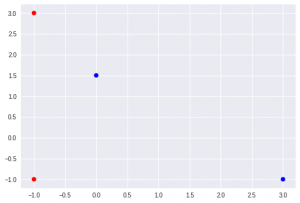
\includegraphics[height=0.3\textheight]{../../Images/ex2_data_halfspace.png}
\end{frame}

%%%%
\begin{frame}
    \frametitle{Example, continued}
    A simple example in $\mathbb R^2$, with $n=4$ points.

    \begin{center}
    \ttt{x}: $\begin{bmatrix}-1 & 3 \\ -1 & -1 \\ 3 & -1 \\ 0 & 1.5\end{bmatrix}$  \qquad\qquad
    \ttt{y}: $\begin{bmatrix}-1 \\ -1 \\ 1 \\ 1\end{bmatrix}$
    \end{center}

    Use $\tilde{\bf w}^{(t)}$ for value of $\tilde{\bf w}$ on step $t$. Start: $\tilde{\bf w}^{(1)} = (0,0,0)$. \newline 
    Next step: $\tilde{\bf w}^{(2)} = \vec{0} + y_1\tilde{\bf x}_1 = -1\ast(1,-1,3) = (-1,1,-3)$.
    \pause
    
    Next: since $y_1\tilde{\bf w}^{(2)}\cdot \tilde{\bf x}_1 > 0$, check $y_2\tilde{\bf w}^{(2)}\cdot \tilde{\bf x}_2 = -1\ast(-1 -1 + 3) = -1$. \pause
    So, 
        \[\tilde{\bf w}^{(3)} = \tilde{\bf w}^{(2)} + y_2\tilde{\bf x}_2 = (-2, 2, -2).\]
    \pause 
    Continue in this way {--} on each step check dot products (in order) with $y_1\tilde{\bf x}_1, y_2\tilde{\bf x}_2, y_3\tilde{\bf x}_3, y_4\tilde{\bf x}_4$. Eventually you return the vector $\tilde{\bf w}^{(10)} = (1, 4, -0.5)$. 
    
    \pause
    i.e., $H = \{(x_1,x_2)\in \mathbb R^2:\ 1 + 4x_1-0.5x_2 = 0\}$ separates the points.
\end{frame}

%%%%
\begin{frame}
    \frametitle{Perceptron algorithm, stopping time}
    Under our assumptions for Perceptron algorithm, a guarantee on eventually stopping.

    \begin{theorem}Define $R = \max_i\lVert\tilde{\bf x}_i\rVert$ and $B = \min\{\lVert{\bf v}\rVert :\  {\bf v} \text{ satisfies }, y_i{\bf v}\cdot \tilde{\bf x}_i \ge 1, \forall i\}$. Then, the Perceptron algorithm stops after at most $(RB)^2$ iterations and, when it stops with output $\tilde{\bf w}$, then $y_i\tilde{\bf w}\cdot \tilde{\bf x}_i > 0$ for all $1\le i\le P$.
    \end{theorem}

    \pause 
    \textbf{Idea of proof:} Write ${\bf v}^*$ for vector that realizes the minimum $B$. Also, $\tilde{\bf w}^{(t)}$ is the vector $\tilde{\bf w}$ on the $t^{th}$ step, $\tilde{\bf w}^{(1)} = (0,0,\ldots,0)$.

    \pause
    Using how $\tilde{\bf w}^{(t+1)}$ is obtained from $\tilde{\bf w}^{(t)}$, can show that ${\bf v}^*\cdot \tilde{\bf w}^{(T+1)} \ge T$ after $T+1$ iterations. Also, using the condition on $\tilde{\bf w}^{(T)}$ that necessitates an update, can show that $|\tilde{\bf w}^{(T+1)}| \le R\sqrt{T}$. (For both statements, induction proves it.) 

    \pause
    With those inequalities and the Cauchy-Schwarz inequality, $T \le BR\sqrt{T}$, which we can rearrange to $T\le (BR)^2$ (if an update was needed on step $T$).
\end{frame}

%%%%
\begin{frame}
    \frametitle{Another example, the Iris data set}
    First discussed by R.A.\ Fisher in a 1936 paper, Iris data set commonly used in explanations. It contains 150 points in $\mathbb R^4$, each for an individual iris flower from one of 3 species: Iris setosa, Iris virginica, and Iris versicolor.

    \onslide<2->{
    The 4 coordinates are measurements of sepal length, sepal width, petal length, and petal width (in cm).
    }

    \onslide<3->{
    Iris setosa points are linearly separable from the other two. \newline 
    Labels: \textit{Iris setosa} $\leftarrow$ 1; \textit{Other species} $\leftarrow$ -1.
    }

    \onslide<4->{
    Begin by opening the notebook \lstinline[language=Python,stringstyle=\ttfamily\color{strings}]{'perceptron-iris-notebook.ipynb'} \ldots 
    After completing the algorithm, should get final $\tilde{\bf w} = (b, {\bf w})$, where ${\bf w} = (1.3,4.1,-5.2,-2.2)$ and $b = 1$.
    }

    \onslide<1->{
    \begin{figure}
    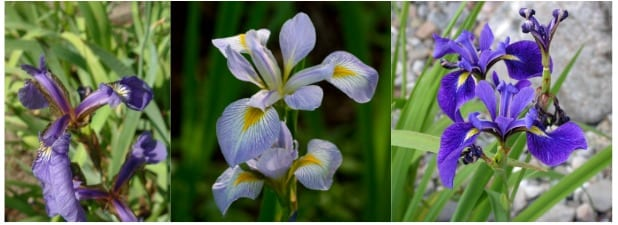
\includegraphics[height=0.2\textheight]{../../Images/iris-3species.jpg}
    \caption{Images by G.\ Robertson, E.\ Hunt, Radomil \copyright CC BY-SA 3.0}
    \end{figure}
    }
\end{frame}
\end{document}